% \textbf{\underline{OZ 3 - De Lorentzkracht en de wet van Ampère - Oefening 3:}}
% \vspace{0.5cm}

% Door een oneindig lange, dikke plaat, die ligt in het $ xy $-vlak en die reikt van $ z = -a $ tot $ z = +a $, loopt een stroomdichtheid $ \vec{J} = c z^2 \hat{\imath} $ met $ c $ een constante. Bepaal het magnetische veld in functie van $ z $, zowel binnen als buiten de dikke plaat.

% \begin{description}[labelwidth=1.5cm, leftmargin=!]
%     \item[Geg. :]   $ z = [-a, a] $;  $ \vec{J} = c z^2 \hat{\imath} $;
% \end{description}

% \begin{figure}[H]
%     \centering
%     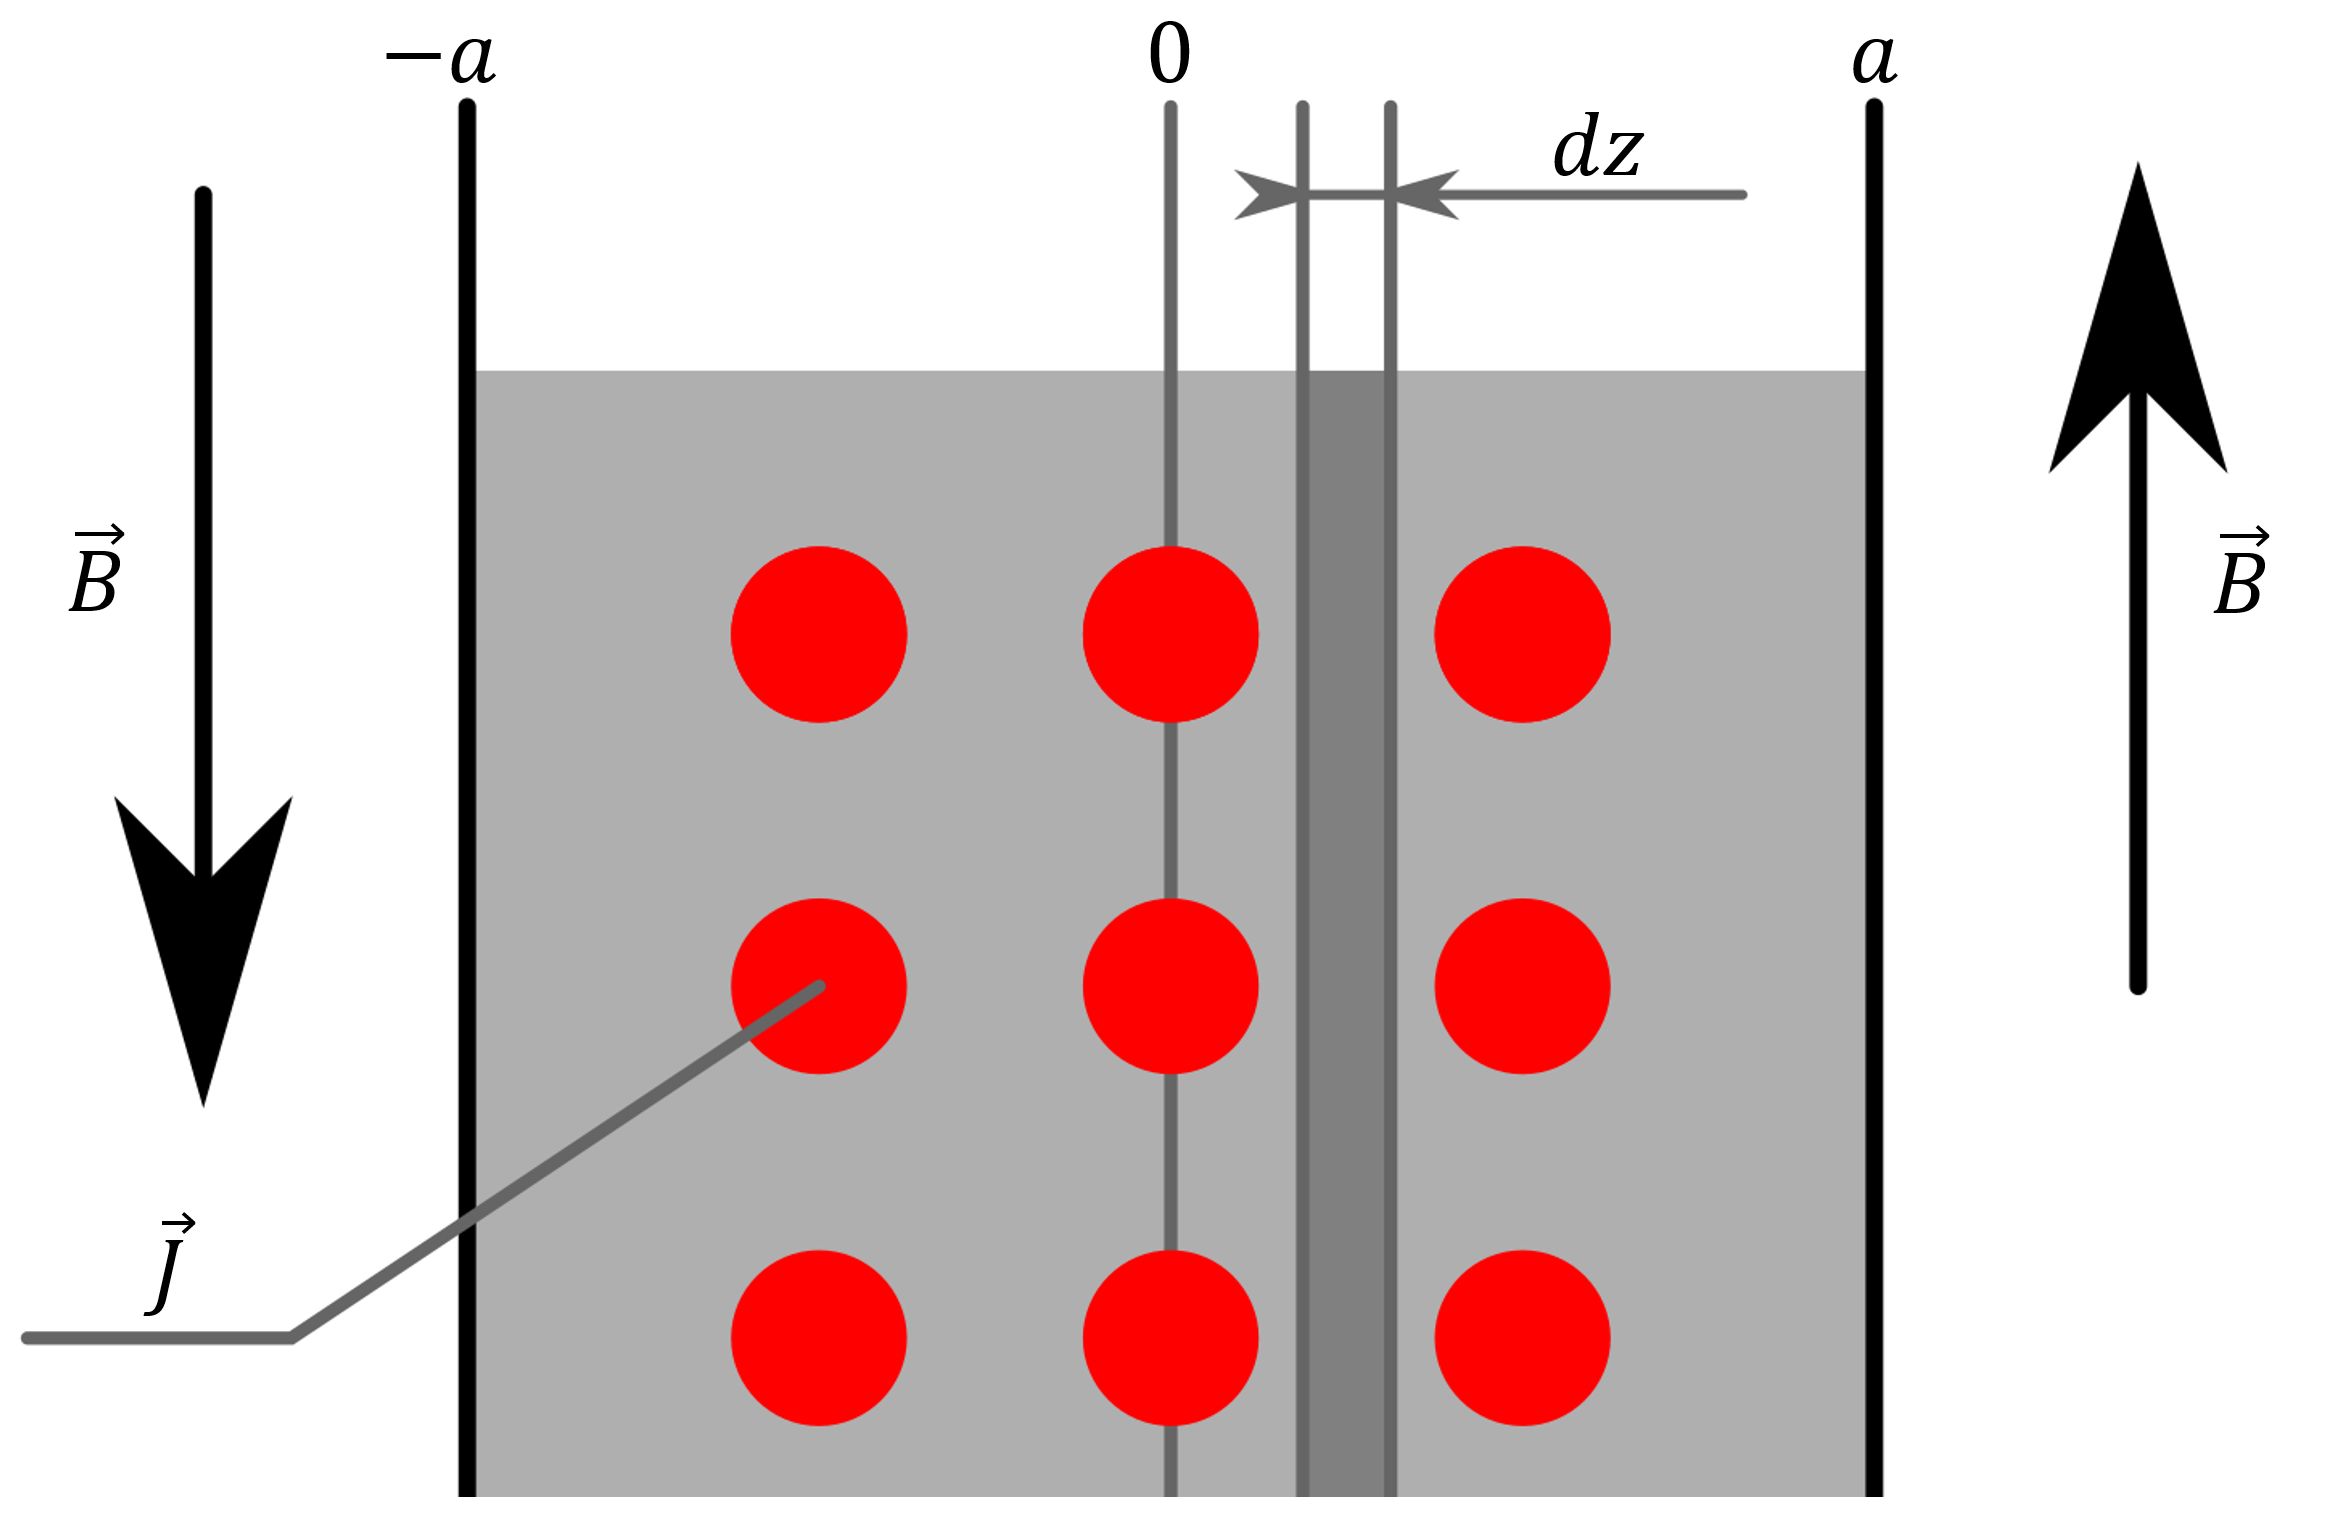
\includegraphics[width=8cm]{oz03/resources/oef-3-schets.png}
    
%     \textbf{Schets 3.2}
% \end{figure}

% \begin{description}[labelwidth=1.5cm, leftmargin=!]
%     \item[Gevr. :]  $ B_{in} $; $ B_{buiten} $;
%     \item[Opl. :]   Als we de dikke plaat opdelen in dunnere platen van dikte $ dz $ kunnen we de plaat beschouwen als een verzameling van dunne stroomvoerende vlakken.
    
%                     Voor het totaal magnetisch veld buiten de plaat te vinden kunnen we integreren over de totale dikte van de plaat:
    
%                     $ B_{buiten} = \int_{-a}^{a}{\dfrac{\mu_0 J}{2} dz} 
%                     = 2 \int_{0}^{a}{\dfrac{\mu_0 c z^2}{2} dz} 
%                     = 2 \left[ \dfrac{\mu_0 c z^3}{6} \right]_{0}^{a} 
%                     = \dfrac{\mu_0 c a^3}{3} $
                    
%                     \vspace{0.5cm}
                    
%                     Voor het magnetisch veld in de plaat moeten we kijken naar wat er links van $ dz $ overblijft, dit zorgt voor een opwaarts veld, en wat er rechts van $ dz $ overblijft, dit zorgt voor een neerwaarts veld (beide in perspectief van de schets).
                    
%                     $ B_{in} = B_{links} - B_{rechts}  $
                    
%                     \hspace{0.55cm} $
%                     = \int_{-a}^{z}{\dfrac{\mu_0 J}{2} dz} - \int_{z}^{a}{\dfrac{\mu_0 J}{2} dz} $
                    
%                     \hspace{0.55cm} $
%                     = \int_{-a}^{z}{\dfrac{\mu_0 c z^2}{2} dz} - \int_{z}^{a}{\dfrac{\mu_0 c z^2}{2} dz} $
                    
%                     \hspace{0.55cm} $
%                     = (\int_{0}^{a}{\dfrac{\mu_0 c z^2}{2} dz} + \int_{0}^{z}{\dfrac{\mu_0 c z^2}{2} dz}) - (\int_{0}^{a}{\dfrac{\mu_0 c z^2}{2} dz} - \int_{0}^{z}{\dfrac{\mu_0 c z^2}{2} dz}) $
                    
%                     \hspace{0.55cm} $
%                     = 2 \int_{0}^{z}{\dfrac{\mu_0 c z^2}{2} dz} $
                    
%                     \hspace{0.55cm} $
%                     = 2 \left[ \dfrac{\mu_0 c z^3}{6} \right]_{0}^{z} $
                    
%                     \hspace{0.55cm} $
%                     = 2 \dfrac{\mu_0 c z^3}{6} $
                    
%                     \hspace{0.55cm} $
%                     = \dfrac{\mu_0 c z^3}{3} $
% \end{description}

% \vspace{1cm}